Plot the frame G coordinates $(2, -1)_G$ Now express the frame G coordinates $(2, -1)_G$ in the frame M, and confirm that this is the same point by plotting it using the frame M.

\begin{solution}
\begin{align*}
    R_{MG} &= \begin{bmatrix}
        \boldsymbol{\hat{i}}_G \boldsymbol{\hat{i}}_M & \boldsymbol{\hat{j}}_G \boldsymbol{\hat{i}}_M \\
        \boldsymbol{\hat{i}}_G \boldsymbol{\hat{j}}_M & \boldsymbol{\hat{j}}_G \boldsymbol{\hat{j}}_M \\
    \end{bmatrix} \\
    &= \begin{bmatrix}
        \frac{1}{2} & \frac{\sqrt{3}}{2} \\
        -\frac{\sqrt{3}}{2} & \frac{1}{2} \\
    \end{bmatrix} \\
    r_M &= R_{MG} r_G \\
    &= \begin{bmatrix}
        \frac{1}{2} & \frac{\sqrt{3}}{2} \\
        -\frac{\sqrt{3}}{2} & \frac{1}{2} \\
    \end{bmatrix} \begin{bmatrix}
        2 \\ -1
    \end{bmatrix} = \begin{bmatrix}
        0.134 \\ -2.232
    \end{bmatrix} \\
    r_M &= 0.134 \boldsymbol{\hat{i}}_M - 2.232 \boldsymbol{\hat{j}}_M
\end{align*}

\begin{center}
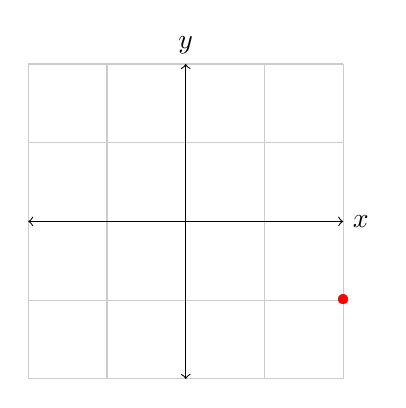
\begin{tikzpicture}
    \draw[thin,gray!40] (-2,-2) grid (2,2);
    \draw[<->] (-2,0)--(2,0) node[right]{$x$};
    \draw[<->] (0,-2)--(0,2) node[above]{$y$};
    \node [red] at (2, -1) {\textbullet};
\end{tikzpicture}
\end{center}
\end{solution}